\begin{tikzpicture}
\draw[black] (0,0) -- (0,8);
\draw[black] (0,0) -- (10,0);
\draw[gray] (0,8) parabola (8,0);
\draw[gray] (0,0) parabola (8,8);
\draw[black] (4,-0.5) node[anchor=west] {Time};
\draw[black] (-0.75,3.5) node[anchor=west] {\begin{turn}{90} $Potential \ and \ Kinetic \ Energy$ \end{turn} };
\end{tikzpicture}

Kinetic energy is the so-called energy of motion. This means that when an object is moving, it  will have a certain amount of energy associated with this motion. To be more specific, Kinetic Energy is the energy gained by an object when a conservative force does work on an object. So when a certain amount of work is done on an object by this conservative force, we would expect the kinetic energy of the force to increase or decrease in turn. We can see this if we look at the expression for work. Work is $$\int{\vec{F} \cdot d\vec{r}}$$ By the second law, this is just $$\int{m\vec{a} \cdot d\vec{r}}$$ But $a=\vec{dv}{dt}$ so we can replace that here $$\int{m\frac{dv}{dt} \cdot d\vec{r}}$$ Now we are going to do something not mathematically rigorous but that physicists use all the time and will work fine for our purposes. That is, we are going to say that we can move from under the $dt$ from the $d\vec{v}$ to the $d\vec{r}$. It is if we are treating $dt$ as just another number that we can multiply. Once again, this is not rigorous, but if you think about $dt$ as just a number, you should see why this makes intuitive sense. Now we can substitute $$\frac{d\vec{v}}{dt}d\vec{r}$$ for $$\frac{d\vec{r}}{dt}d\vec{v}$$ But $\frac{dr}{dt}$ is is just $\vec{v}$. So we can rewrite our integral as $\int{mv d\vec{v}}$. When we integrate we use the power rule and then substitute at two velocities to find that find that \begin{equation}W=\Delta\left(\frac{mv^2}{2}\right)\end{equation} we have said that kinetic energy is the change associated in the energy of an object when work is performed on it so from Eqn. 3.4.1 it is clear that $\frac{mv^2}{2}$ is just what we are looking for. Kinetic Energy is often denoted as K, and its units are the same as those of work, Joules. \begin{equation}K=\frac{mv^2}{2}\end{equation} The connection between work and energy that we have just derived is called the work-energy theorem. The work-energy theorem states that \begin{equation}W_{conservative}=\Delta K\end{equation} When I first learned this formula I was amazed because it seemed magical that this term we had created was exactly what we needed in this case. This formula will come in handy in many situations, so it is important that you fully understand it and its derivation. Also, note that this formula can only be applied in one dimension. Because work is a dot product, we would have to use the dot product to find the answer when we have multiple dimensions, and I would challenge you to do this using the same method we have described above. The answer may be less satisfying, but it may help you answer some of the questions you have. Now that we have started talking about the kinetic energy we have to study potential energy. We will study it more rigorously later but for now, think about potential energy as being energy that will later be converted into kinetic energy. So, if a ball is very high, it will have higher potential energy because it will fall farther and hit the ground with a faster speed(and therefore kinetic energy), than a ball that was dropped from a lower height. For our purposes, we only need to consider one type of potential energy this way. That is gravitational potential energy. Essentially, when things get higher in the sky, they get more gravitational potential energy. Likewise, when things get lower, they will lose potential energy. Like always, work and potential energy are closely related. When a conservative force does work on an object(for right now this means gravity), the potential energy of the object will decrease with the same magnitude as the work done on the object. Another way of writing this is that \begin{equation}W_{conservative} = -\Delta U\end{equation} Where $U$ represents the potential energy. All this says is that when gravity does work on an object(by lowering its position), the potential energy of the object will decrease by the same amount. Think about this if you have trouble with it because we will use this definition very often. Now let us think about what happens when the gravitational force does work on an object. The first thing to note is that we can consider the gravitational force to be directly down. This means that if an object moves to the right or left, the gravitational force is not responsible for this movement. So let us think about the work done by gravity on an object that moved down a height $h$. The work done will be $mgh$. This is because the direction of the motion(downwards), and the force of gravity(also downwards), are the same, so the angle is 0 and $\cos\left(\theta \right)=1$. Also, the force is $mg$ and is constant, and the height moved downward is $h$. The product is $mgh$. Therefore if the work is done is $mgh$, the potential energy has decreased by $mgh$ in turn. The opposites would be true if the object went up by a height h. The work done would be $-mgh$, and the potential energy would increase by $mgh$. Hopefully, this will not be too confusing but you should not that I have only defined what a change in potential energy entails and not what the exact value of potential energy is. That is because for what we are doing right now, we can define the absolute value of the potential energy however we would like. For example, if we have an object at a height h above the earth at $t_1$ and the same object on the ground at $t_2$. We could define the potential energy of the object at $t_2$ as 0, and the energy of the object at $t_1$ as $mgh$. This is because the work done by gravity in bringing the object from height h to the ground is $mgh$, so the potential energy from height $h$ to the ground decreases by $mgh$ and therefore the ball must have potential energy greater at height h by $mgh$. However, it is not necessary that this value be $mgh$. All that matters is that the difference in potential energies is $mgh$. So, we could say the potential energy at height $h$ is $2mgh$ and at the ground is $mgh$ . Once again, all that matters is the difference. We will see this one more time when discussing electric potential. Now that we understand potential and kinetic energy, we need to understand the relationship between the two; this comes in the form of conservation of energy. Essentially, the first thing we need to know about conservation of energy is that \begin{equation}K_1+U_1=K_2+U_2\end{equation} if only conservative forces are acting on the system with the energy. Simplifying this we can write that $$\Delta U+\Delta K=0$$ when the only forces acting on the object are conservative. You can get this formula yourself by plugging in the values we have given for $\Delta U$ and $\Delta K$ before. It is easy to see now that we have written the formula for the conservation of energy in this way, what the formula should be when we have non-conservative forces acting on the object. All you need to know about conservative and non-conservative forces now is that gravity is the only conservative force of importance. So anything else will be non-conservative. Essentially, non-conservative forces take energy or add energy to a system, while conservative forces cannot do this. So we can write that \begin{equation}\Delta U+\Delta K=W_{non-conservative}\end{equation} where $W_{non-conservative}$ is the work done on the system(or just object) by the non-conservative force. To illustrate this concept, we will do one example that encompasses all of the topics we have learned about. This is just a block sliding down a frictional plane, as seen in Fig. 4.3.1. Our task is to find out what the velocity of the object will be once it gets to the bottom of the plane. We will be given the angle of the frictional plane, the length of the place, the frictional constant, and the mass of the object. 

Also, we can assume that the object essentially only occupies the exact top of its current location, so we do not have to worry about the fact that it is not completely at this top. This assumption from now is often implicitly made but will not be stated. Also, we assume the mass is at rest at the top of the ramp. We use Eqn. 4.3.6. 
\newline
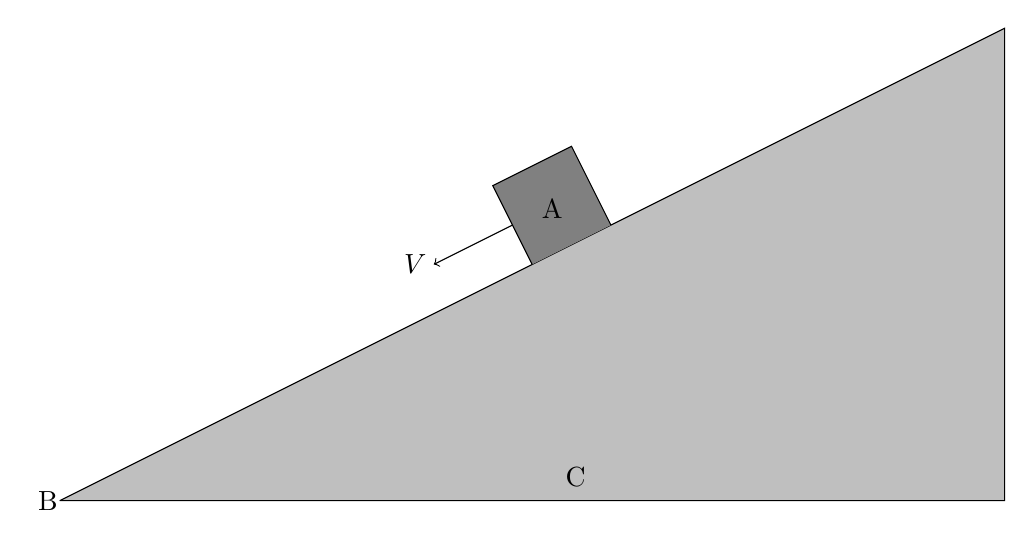
\begin{tikzpicture}
\filldraw[draw = black, fill = lightgray] (0,0) -- (12,0) -- (12,6) -- (0,0);
\filldraw[draw = black, fill = gray] (6,3) -- (5.5,4) -- (6.5,4.5) -- (7,3.5);
\draw[black, ->] (5.75,3.5) -- (4.75,3);
\draw[black] (4.25,3) node[anchor=west] {$V$};
\draw[black] (6,3.7) node[anchor=west] {A};
\draw[black] (6.3,0.3) node[anchor=west] {C};
\draw[black] (-0.4,0) node[anchor=west] {B};
\end{tikzpicture}
\newline
\begin{center}
(Figure 4.3.1)
\end{center}
$$\Delta U+\Delta K=W_{non-conservative}$$ Here, friction will be the non-conservative force. We can calculate what $W_{non-conservative}$ is at the beginning. The normal force is $$mg\cos\left(\theta \right)$$ Therefore the force of friction is $\mu mg\cos\left(\theta \right)$ in the direction up the ramp because the mass is going down the ramp. So the work done by friction is $$\vec{F} \cdot \vec{d}=\mu mgh\cos\left(\theta_1 \right)$$ Here $\theta_1$ is the angle between the force of friction and the direction of motion of the mass. $\theta_1$ is 180 degrees so $cos\left(\theta_1 \right)=-1$ and therefore,  $$W_{non-conservative}=-\mu mgh\cos\left(\theta_1 \right)=\Delta U+\Delta K$$ Next, let us examine the change in kinetic energy. The kinetic energy of the object at the top of the ramp is 0(it is at rest) as. So, $$\Delta K=\frac{mv^2}{2}$$ In this example, and many other examples, the kinetic energy term will allow us to find the velocity of the object. Next, we need to find the change in potential energy of the object between the top and bottom of the ramp. Remember that $$W_{conservative}=-\Delta U$$ So, if we find the work done by gravity in moving the mass from the top to the bottom of the ramp, we will be able to find the change in potential energy of the object. We are going to use something special about conservative forces to find the work done by gravity here. That is, we will use the fact that conservative forces are path-independent. So, the work done by gravity in taking it from point A to point B will be the same as if we took the object from point A, directly down to the bottom of the ramp to point C, and then directly to the right to point B. In moving the object from point C to point B, gravity does no work because it is directly perpendicular to the motion of the object. Meanwhile, gravity does do work while moving the object from point A to point C. And when moving it from A to C, the force of gravity and the direction of motion of the object is in the same direction so $$W_{gravity}=mg\left(distance\ from\ point\ A\ to\ point\ C \right)$$ Using trigonometry(I recommend you do this yourself), we can find that the distance from point A to point $C=h\sin\left(\theta \right)$. Therefore \begin{equation}W_{gravity}=mgh\sin\left(\theta \right)\end{equation} Finally, we have \begin{equation}\Delta U=-mgh\sin\left(\theta \right)\end{equation} So, we can now finally find the velocity we are looking for. $$-\mu mgh\cos\left(\theta \right)=-mgh\sin\left(\theta \right)+\frac{mv^2}{2}$$ We can rearrange this equation to find that $$mg\left(\sin\left(\theta \right )-\mu \cos\left(\theta \right)\right)=\frac{mv^2}{2}$$ Therefore \begin{equation}v=\sqrt{\left(2mgh\left(\sin\left(\theta \right)-\mu \cos\left(\theta \right)\right)\right)}\end{equation} You may be confused as to what happens when $$\sin\left(\theta \right)-\mu \cos\left(\theta \right) < 0$$ If this were the case, the velocity would be an imaginary number. Well, do not worry. This is not possible. If $$\sin\left(\theta \right)-\mu \cos \left(\theta \right) < 0$$ then object will not move initially and our formula will not apply. I challenge you to justify this for yourself using Newton’s laws. 